\documentclass[12pt]{article}
\usepackage{times} 			% use Times New Roman font

\usepackage[margin=1in]{geometry}   % sets 1 inch margins on all sides
\usepackage{hyperref}               % for URL formatting
\usepackage[pdftex]{graphicx}       % So includegraphics will work
\setlength{\parskip}{1em}           % skip 1em between paragraphs
\usepackage{indentfirst}            % indent the first line of each paragraph
\usepackage{datetime}
\usepackage[small, bf]{caption}
\usepackage{listings}               % for code listings
\usepackage{xcolor}                 % for styling code
\usepackage{multirow}
\usepackage{xurl} 
\usepackage{enumitem}
\usepackage[section]{placeins}
\usepackage{float}
\usepackage{hyperref}

%New colors defined below
\definecolor{backcolour}{RGB}{246, 246, 246}   % 0xF6, 0xF6, 0xF6
\definecolor{codegreen}{RGB}{16, 124, 2}       % 0x10, 0x7C, 0x02
\definecolor{codepurple}{RGB}{170, 0, 217}     % 0xAA, 0x00, 0xD9
\definecolor{codered}{RGB}{154, 0, 18}         % 0x9A, 0x00, 0x12

%Code listing style named "gcolabstyle" - matches Google Colab
\lstdefinestyle{gcolabstyle}{
  basicstyle=\ttfamily\small,
  backgroundcolor=\color{backcolour},   
  commentstyle=\itshape\color{codegreen},
  keywordstyle=\color{codepurple},
  stringstyle=\color{codered},
  numberstyle=\ttfamily\footnotesize\color{darkgray}, 
  breakatwhitespace=false,         
  breaklines=true,                 
  captionpos=b,                    
  keepspaces=true,                 
  numbers=left,                    
  numbersep=5pt,                  
  showspaces=false,                
  showstringspaces=false,
  showtabs=false,                  
  tabsize=2
}

\lstset{style=gcolabstyle}      %set gcolabstyle code listing

\makeatletter
\g@addto@macro{\UrlBreaks}{\UrlOrds}
\makeatother

% for fancy page headings
\usepackage{fancyhdr}
\setlength{\headheight}{13.6pt} % to remove fancyhdr warning
\pagestyle{fancy}
\fancyhf{}
\rhead{\small \thepage}
\lhead{\small HW3, Lewis}  
\chead{\small CS 432, Fall 2020} 

%-------------------------------------------------------------------------
\begin{document}

\begin{centering}
{\large\textbf{HW3 - Ranking Web Pages}}

Brenden Lewis\\                     
Due: 10/18/2020 11:59PM\\                      
\end{centering}

%-------------------------------------------------------------------------
\section*{Q1}
Unfortunately, I had to acquire a brand new set of URIs to use for this assignment due to my dataset from HW\#2 being comprised almost entirely of YouTube links; these kinds of links provide very little in terms of HTML content. For the sake of time, I only collected about 750 URIs through the Twitter API. I used a variety of keywords related to \emph{tech} and \emph{current events} in an attempt to broaden the contents of each page and provide a larger dictionary of words to utilize for this assignment. Unlike in my HW\#2 submission, I was able to eliminate duplicates in my set and was left with 740 URIs before processing; these URIs were passed in as \emph{CleanedURLs.txt}. 

There were a few issues with some URIs throwing unique errors that I had to exempt due to not knowing how to work around. One of example of this was a link to a working Amazon page that was throwing a weird 503 error. After a bit of research, in this case, it was due to Amazon having their own API (similar to TWitter) that's required to scrape their data. 

\par I downlaoded the HTML for each URI using the \emph{requests} library and processed the HTML using \emph{boilerpipe.extract} to extract the primary text. The raw HTML and processed text per URI was automatically stored in their own \emph{.txt} files and saved in a local directory using a counter to label file names. This apporach resulted in a \emph{rawHTMLFile\#.txt} and \emph{processedHTMLFile\#.txt} file combo per URI stored in seperate folders locally.

\lstinputlisting[language=Python, caption=Python code for downloading and processing html, label=lst:import]{q1.py}

\section*{Q2}

I opted to make a Python script specifically for sorting through my data set and collecting URIs that contained a specific query (as shown in Listing 2 below). Due to a large portion of my URIs being related to games and game companies, I chose the query "Xbox" for collecting URIs to use in ranking later. In order to read through all the processed files I had stored, I used both the \emph{glob} and \emph{os} libraries in conjunction with the path to folder. For each file, text was read line-by-line, word-by-word to check for any matches to the query. To help with ranking the URIs later on, I was keeping count of each time the query was found in a file and the total amount of words the file possessed. Each file was stored as a dictionary with this information including the file name, and written to \emph{QueryResults.txt} if the query ever appeared in the file.

\lstinputlisting[language=Python, caption={Python code for collecting URIs that contain the query, query frequency, and total word count per document}, label=lst:import]{countQuery.py}

With the query set to 'Xbox', 24 files were found to contain the query out of the 740. The output from this operation is shown Listing 3. Listing 3 shows 701 total documents because after running it the first time, I discovered that a good chunk of rawHTML and processedHTML files collected from Q1 were either empty or nearly empty (either 0 or 1 kb). I decided to delete those entries and run it again for the sake of consistency and not having missing data (GitHub won't allow uploading of empty files). 

\begin{lstlisting}[language=Python, caption={QueryResults.txt}, label=lst:copy]
Query: Xbox
{'file': 'processedHtmlFile1.txt', 'words:': 412, 'occurences': 8}
{'file': 'processedHtmlFile103.txt', 'words:': 256, 'occurences': 8}
{'file': 'processedHtmlFile106.txt', 'words:': 407, 'occurences': 4}
{'file': 'processedHtmlFile11.txt', 'words:': 581, 'occurences': 11}
{'file': 'processedHtmlFile110.txt', 'words:': 407, 'occurences': 4}
{'file': 'processedHtmlFile119.txt', 'words:': 587, 'occurences': 11}
{'file': 'processedHtmlFile12.txt', 'words:': 481, 'occurences': 11}
{'file': 'processedHtmlFile120.txt', 'words:': 407, 'occurences': 4}
{'file': 'processedHtmlFile122.txt', 'words:': 252, 'occurences': 4}
{'file': 'processedHtmlFile123.txt', 'words:': 450, 'occurences': 4}
{'file': 'processedHtmlFile13.txt', 'words:': 225, 'occurences': 4}
{'file': 'processedHtmlFile15.txt', 'words:': 138, 'occurences': 2}
{'file': 'processedHtmlFile194.txt', 'words:': 1247, 'occurences': 1}
{'file': 'processedHtmlFile2.txt', 'words:': 48, 'occurences': 1}
{'file': 'processedHtmlFile235.txt', 'words:': 423, 'occurences': 1}
{'file': 'processedHtmlFile3.txt', 'words:': 213, 'occurences': 1}
{'file': 'processedHtmlFile4.txt', 'words:': 496, 'occurences': 6}
{'file': 'processedHtmlFile5.txt', 'words:': 207, 'occurences': 2}
{'file': 'processedHtmlFile6.txt', 'words:': 55, 'occurences': 1}
{'file': 'processedHtmlFile740.txt', 'words:': 323, 'occurences': 4}
{'file': 'processedHtmlFile8.txt', 'words:': 276, 'occurences': 7}
{'file': 'processedHtmlFile96.txt', 'words:': 326, 'occurences': 5}
{'file': 'processedHtmlFile97.txt', 'words:': 97, 'occurences': 2}
{'file': 'processedHtmlFile99.txt', 'words:': 212, 'occurences': 5}

Total # of documents: 701
Total # of documents that contain query: 24
\end{lstlisting}

I searched through each file to determine which would be best to use for calculation; this was based on a combination of factors such as content, size, language (several were in Portugese, only opted to include one), and which ones I was curious to see the results of. The final 10 I chose to analyze are listed below in Listing 4. I had to manually add in the URLs for each of the 10 to make things a little easier when putting everything together in the end.

\begin{lstlisting}[language=Python, caption={Final set of 10 URIs chsoen for TD-IDF calculations}, label=lst:copy]
{'file': 'processedHtmlFile1.txt', 'uri': 'https://www.resetera.com/threads/xbox-brasil-dismisses-new-host-after-she-was-the-victim-of-death-and-rape-threats.307873/', 'words': 412, 'occurences': 8}
{'file': 'processedHtmlFile103.txt', 'uri': 'https://www.theverge.com/2020/10/15/21517293/xbox-series-x-s-dashboard-ui-october-update-release?_lrsc=f9510bb1-a7e2-43c8-9e49-761f32bbdc52', 'words': 256, 'occurences': 8}
{'file': 'processedHtmlFile2.txt', 'uri': 'https://www.exophase.com/user/toniazzo/?1602892894', 'words': 48, 'occurences': 1}
{'file': 'processedHtmlFile194.txt', 'uri': 'https://newszoneweb.com/?p=5809','words': 1247, 'occurences': 1}
{'file': 'processedHtmlFile106.txt', 'uri': 'https://www.gamespot.com/articles/future-bethesda-titles-dont-need-to-be-on-ps5-says-xboxs-phil-spencer/1100-6483415/', 'words': 407, 'occurences': 4}
{'file': 'processedHtmlFile740.txt', 'uri': 'https://www.gamespot.com/articles/marvels-avengers-ps5-and-xbox-series-x-s-versions-delayed-to-2021/1100-6483398/', 'words': 323, 'occurences': 4}
{'file': 'processedHtmlFile12.txt', 'uri': 'https://tictechbuzz.com/remembering-the-classics-the-xbox-podcast-featuring-tim-schafer/', 'words': 481, 'occurences': 11}
{'file': 'processedHtmlFile8.txt', 'uri': 'https://g1.globo.com/pop-arte/games/noticia/2020/10/16/microsoft-demite-apresentadora-do-xbox-br-que-sofreu-ameacas.ghtml?utm_source=twitter&utm_medium=social&utm_campaign=g1', 'words': 276, 'occurences': 7}
{'file': 'processedHtmlFile13.txt', 'uri': 'https://www.engadget.com/lucasarts-double-fine-remasters-game-pass-235238100.html', 'words': 225, 'occurences': 4}
{'file': 'processedHtmlFile119.txt', 'uri': 'https://www.ign.com/articles/phil-spencer-xbox-bethesda-ps5?utm_source=dlvr.it&utm_medium=twitter', 'words': 587, 'occurences': 11}
\end{lstlisting}

The Python code for calculating TF-IDF values (Listing 5) was relatively straight forward. I had to utilize the \emph{ast} library to pull in the information from \emph{FinalURLsForRanking.txt} as dictionaries to be used. I was using Google as my corpus, so that variable for calculation was 55b. The TF, IDF, and TF-IDF values were each calculated in their own individual function to 3 significant figures to reduce clutter. The \emph{form operator import itemgetter} was needed to sort my final data in descending order by TF-IDF value; this wasn't completely necessary with how I created my table, but it definitely helped speed-up the process.

\lstinputlisting[language=Python, caption=Python code for calculating the TF-IDF for each URI, label=lst:import]{RankingURls.py}

Figure 1 below shows the final ranking for each URI and their calculated TF, IDF, and TD-IDF values. For both the TD-IDF table and PageRank tables, I opted to use Excel to show the results as with only a few entries I didn't mind doing it manually. Looking at the results, an article from The Verge had the highest TF ratio of 8/256 which resulted in a larger TF-IDF. This is interesting as it ranked higher than the \url{https://tictechbuzz.com} link, which I expected to be the highest due to a higher query count; it had a larger query frequency, but also more total words at 11/481, resulting in a lower TF-IDF value. The lowest recorded value only had a single occcurence of the query over 1247 words. I was expecting it to be lower than every other URI, but I was still curious how low of a value would be calculated.  

\begin{figure}[H]
            \centering
            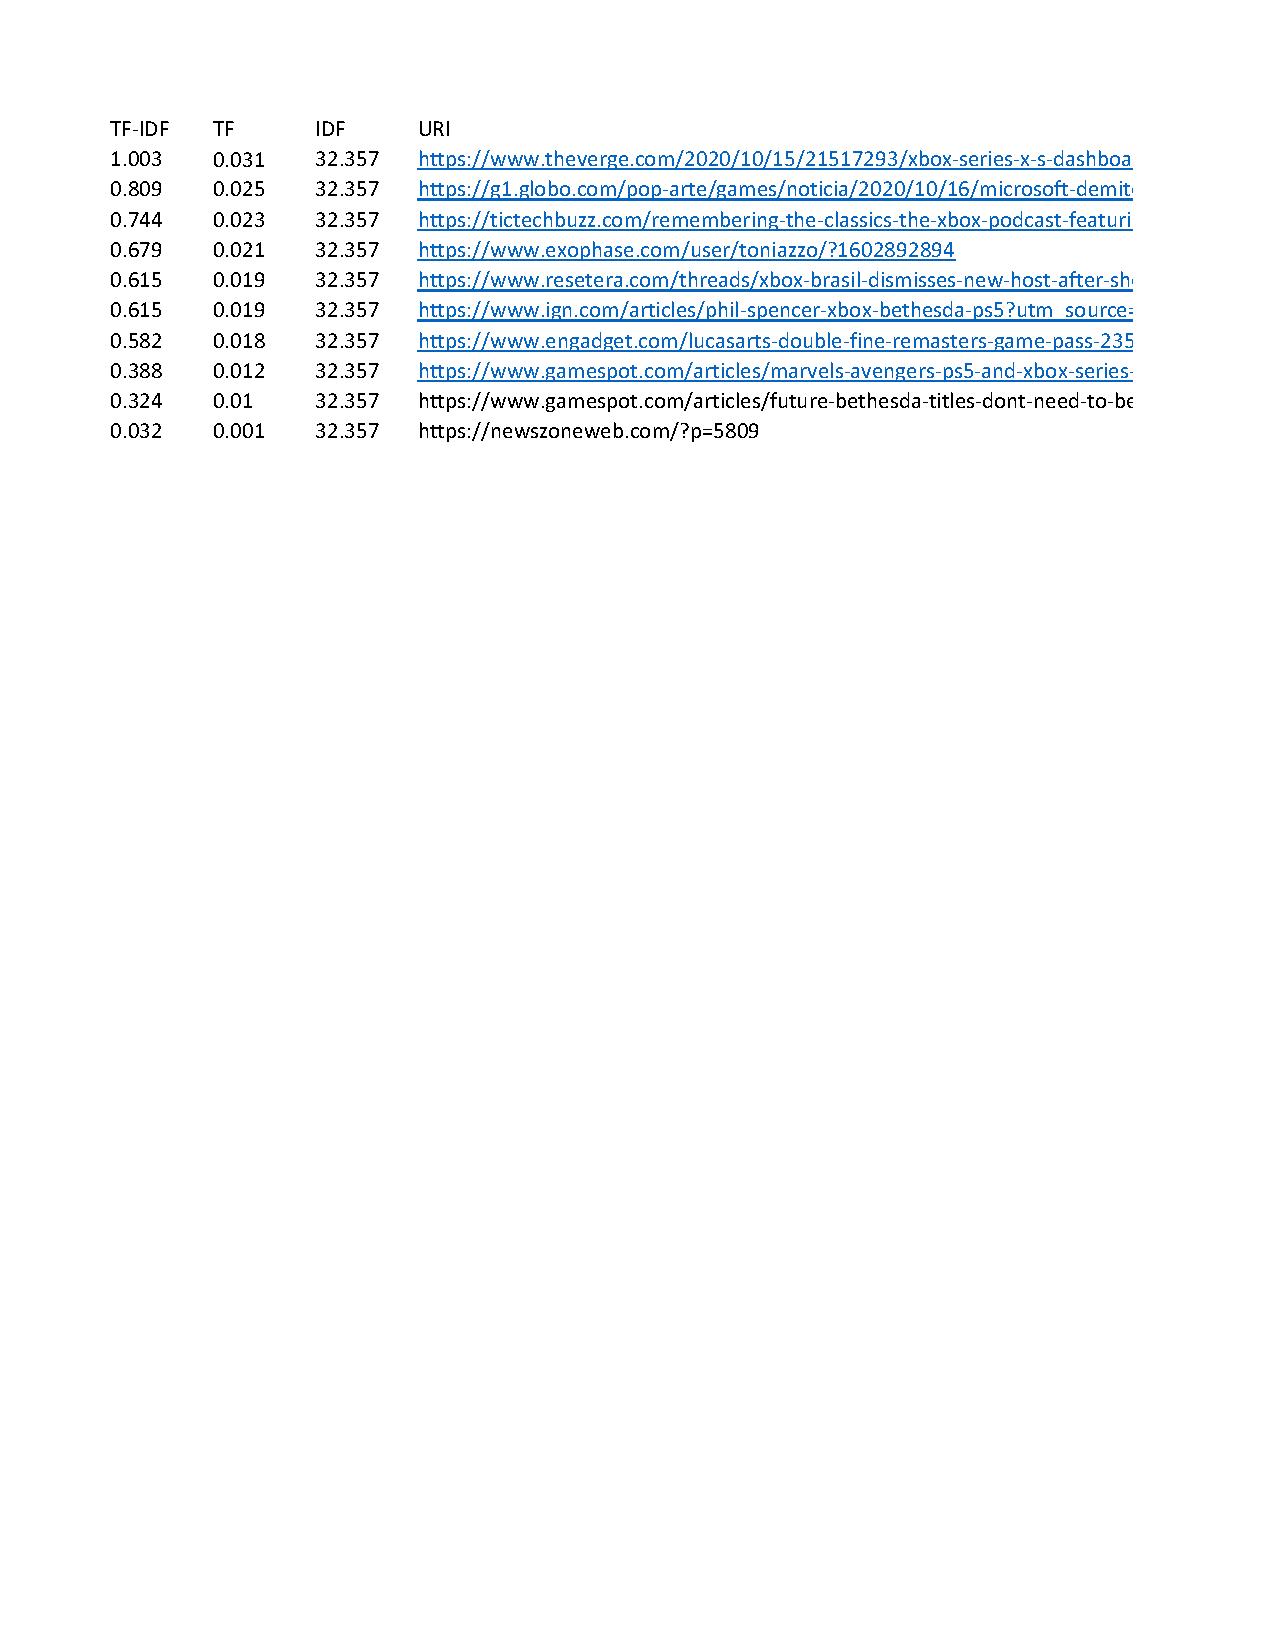
\includegraphics[trim = 0 20cm {0.31\textwidth} 2cm, clip]{TF_IDF_Table.pdf}
            \caption{Chart showing the TF-IDF, TF, and IDF for the query 'Xbox' across 10 chosen URIs}
            \label{fig:my_label}
        \end{figure}


\section*{Q3}

Figure 2 below shows the PageRank ranking for each URI. Each URI was checked using \url{https://www.prchecker.info/check_page_rank.php}. Unfortunately, due to these being obscure pages, every single URI returned with a 0/10 ranking as per the PR estimater. This is a sharp contrast to the TD-IDF table. I was a expecting a few URIs to have some kind of rank given their TD-IDF values, but was met with zeros across the board.

\begin{figure}[H]
            \centering
            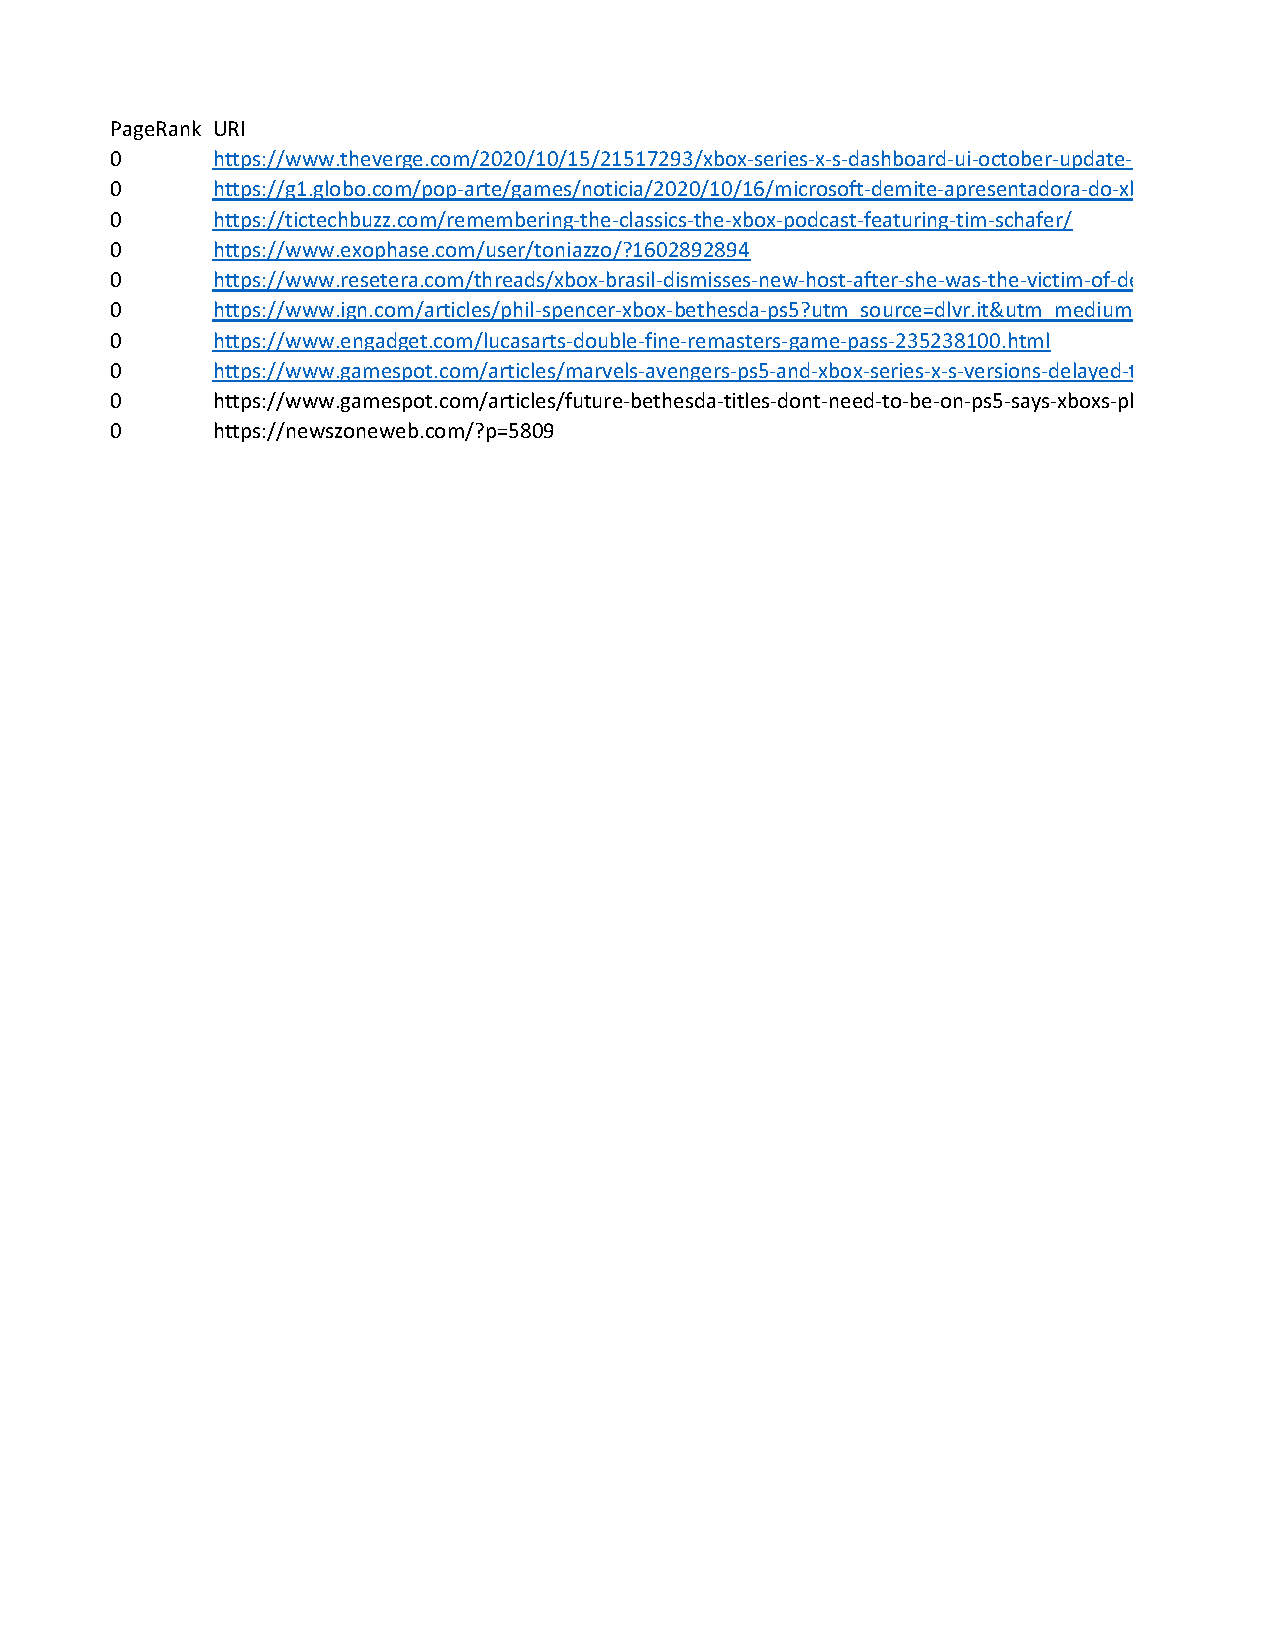
\includegraphics[trim = 0 20cm {0.31\textwidth} 2cm, clip]{PageRank_Table.pdf}
            \caption{Chart showing the results of ranking each URI with PageRank}
            \label{fig:my_label}
        \end{figure}

\end{document}
